\documentclass[]{article}
\usepackage{graphicx}
%opening
\title{LiRX V1}
\author{}
\date{}

\begin{document}

\maketitle

\begin{abstract}
	LiRX - Licht Receiver.
	
		
	
	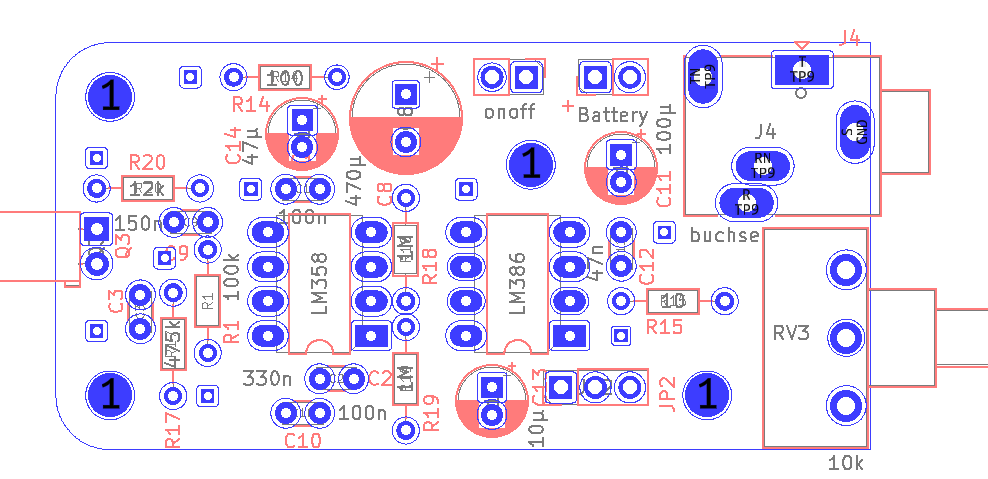
\includegraphics[width=1.0\linewidth]{Platine.png}
Liste der elektronischen Bauteile in aufsteigender Bauhöhe.
\end{abstract}

\section{Widerstände}
\begin{itemize}
	\item R1 :	100k$\Omega$
	\item R14 : 100$\Omega$ - Entkopplung LM358 Stromversorgung
	\item R15 : 10$\Omega$ - Endfilter LM386
	\item R17 : 470k$\Omega$ Feedback Widerstand
	\item R18 : 1M$\Omega$ - Für Spannungsteiler virtual GND 
	\item R19 : 1M$\Omega$ - Für Spannungsteiler virtual GND
	\item R20 : 12k$\Omega$ - Strom für Photosensor
\end{itemize}
\section{Fassungen und Buchse}
\begin{itemize}
	\item 8pol Fassung für LM358
	\item 8pol Fassung für LM386
	\item 3,5mm Klinkenbuchse
\end{itemize}
\section{Kerko Kondensatoren}
\begin{itemize}
	\item C1 : 100nF - Spannungsstabilisation
	\item C2 : 100nF - Spannungsstabilisation
	\item C3 : optional um Oszillation des LM358 zu verringern
	\item C9 : 150nF - Gleichspannung auskoppeln
	\item C10 : 330nF - Gleichspannung auskoppeln
	\item C12 : 47nF - Endfilter LM386
	
\end{itemize}
\section{Elko Kondensatoren}
Auf Polung achten!
\begin{itemize}
	\item C8: 470$\mu$F $\oslash$8mm - Spannungsstabilisation
	\item C11: 100$\mu$F $\oslash$5mm - Entkopplung Audiosignal Gleichstrom
	\item C13: 10$\mu$F $\oslash$5mm - Verstärkungsboost LM386
	\item C14: 47$\mu$F  $\oslash$5mm Spannungsstabilisation
\end{itemize}
\section{Photosensor}
Wahlweise Photodiode oder Phototransistor.

Auf Polung achten, sonst funktioniert es nicht.

Alternativ kann auch jede Leuchtdiode als Photosensor verwendet werden. Ein Photowiderstand wird zu träge sein.
\section{Stromversorgung}
Es gibt einen Anschluss für eine 9V Batterie. Auf Polung achten!

Nach dem Anschluss gibt es zwei Pinlöcher für Nutzung eines Jumper oder zum Anlöten eines Schalters mit Kabel.

\section{Letzte Komponenten}
Für den LM386 ist eine Reihe von drei Pins vorhanden. Wahlweise kann hier ein Jumper oder ein Schalter angelötet werden, um die Verstärkung des LM386 zu vergrößern.

Zuletzt ist RV3 ein 10k$\Omega$ Potentiometer.
\section{Testpunkte}
Auf der Unterseite der Platine sind Testpunkte vorbereitet:

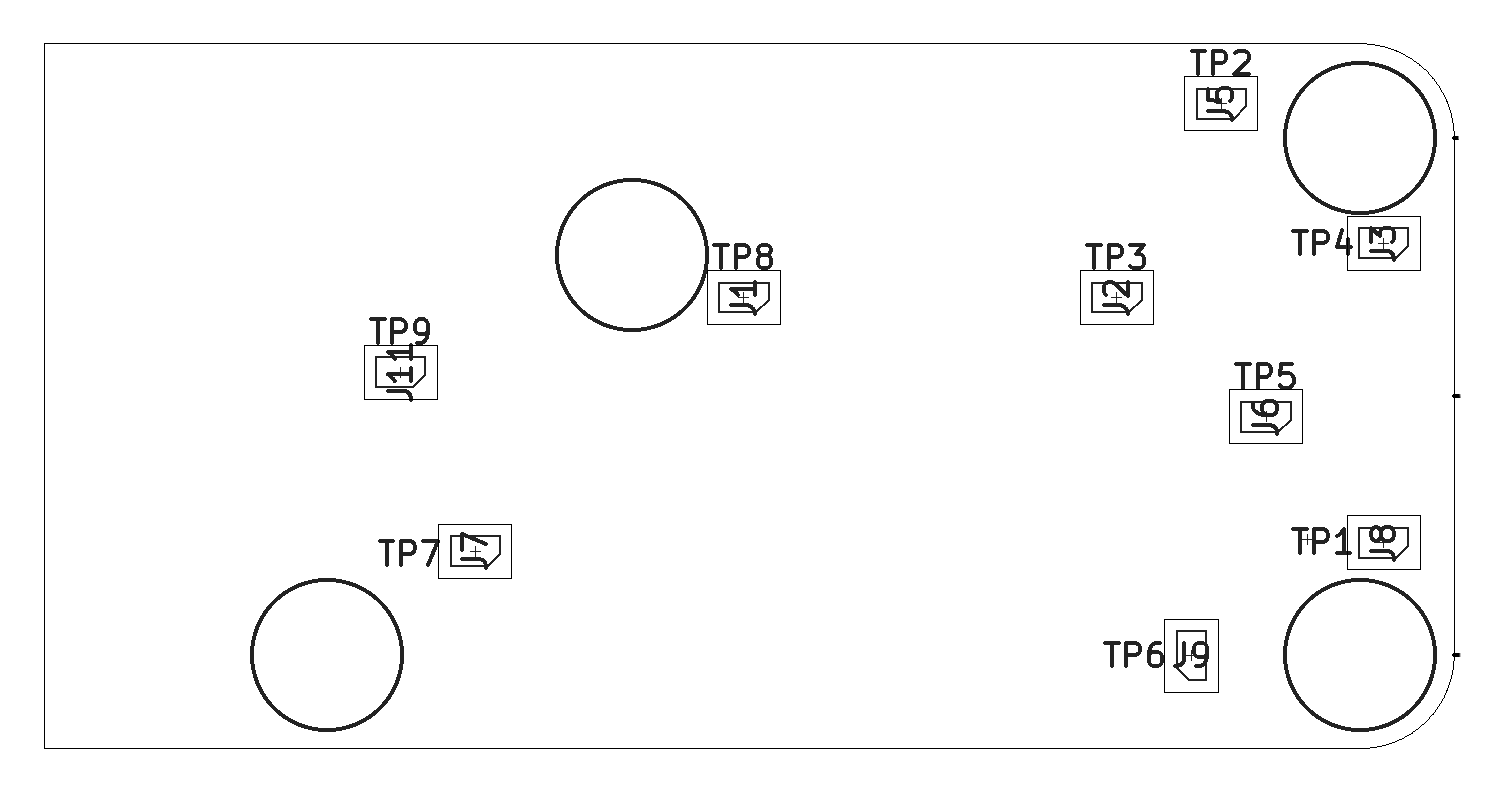
\includegraphics[width=1.0\linewidth]{testpoints.png}

\begin{itemize}
	\item TP1: Ground Pegel, Minuspol Batterie
	\item TP2: Positive Spannung 9V, Pluspol Batterie
	\item TP3: Mittlere Spannung
	\item TP4: Spannung über Photosensor.
	\item TP5: Signal Photosensor nach Kondensator C9
	\item TP6: Signal nach Verstärkung durch Operationsverstärker LM358
	\item TP7: Signal nach Potentiometer.
	\item TP8: Signal direkt nach LM386.
	\item TP9: Signal am Audioausgang.
\end{itemize}
\section{Abschlussbemerkung}
Entstanden auf Impuls von DC3TC ist diese Platine ein Open Source Nachbau des Empfängers des AATIS Projekt AS802 ``Einfacher Licht-Sende-Empfänger (ELiSE)".
DC3TC ist auch der Namensgeber. Das Projekt residiert derzeit hier: https://github.com/dk5ee/LiRX

\end{document}
